

\usetikzlibrary{arrows.meta,calc,patterns,shapes}
\providecommand{\computer}{%
    
\includegraphics[width=1cm]{../common/Noun_project_216.pdf}
}
\providecommand{\switch}{%
    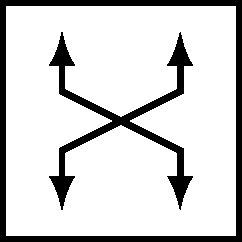
\includegraphics[width=0.9cm]{../common/fig-switch.pdf}
}
\providecommand{\bigswitch}{%
    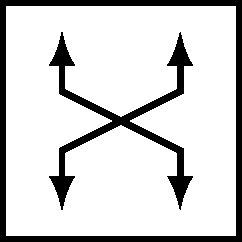
\includegraphics[width=1.4cm]{../common/fig-switch.pdf}
}
\providecommand{\router}{%
    
\includegraphics[width=0.9cm]{../common/fig-router.pdf}
}


\begin{frame}[label=connTwoNet]{two networks in one}
\begin{tikzpicture}
\tikzset{
    connect/.style={draw,very thick,Latex-Latex},
    computer/.style={inner sep=0mm,outer sep=0mm,execute at begin node={\computer}},
    phone/.style={draw,thin,font=\tiny,inner sep=1mm,outer sep=0mm,execute at begin node={phone}},
    switch/.style={inner sep=0mm,outer sep=0mm,execute at begin node={\switch}},
    big switch/.style={inner sep=0mm,outer sep=0mm,execute at begin node={\bigswitch}},
    router/.style={inner sep=0mm,outer sep=-2mm,execute at begin node={\router},circle},
    packet/.style={minimum width=.4cm,minimum height=0.2cm,inner sep=0mm,outer sep=0mm,draw},
    packet lg/.style={minimum width=.6cm,minimum height=0.2cm,inner sep=0mm,outer sep=0mm,draw},
    network/.style={draw,cloud,font=\small,aspect=3,inner sep=-.25cm},
    tunnel/.style={dotted,line width=1mm,dotted,blue,Latex-Latex,opacity=0.7},
}
\begin{scope}
    \node[switch,anchor=south] (switch A) at (2,3) {};
    \node[switch,anchor=south] (switch B) at (4,3) {};
    \node[computer] (c1) at (0,0) {};
    \node[phone] (p1) at (1,0) {};
    \node[computer] (c2) at (2,0) {};
    \node[phone] (p2) at (3,0) {};
    \node[computer] (c3) at (4,0) {};
    \foreach \x/\y in {c1,p1,c2} {
        \draw[connect] (\x) -- (switch A);
    }
    \foreach \x/\y in {p2,c3} {
        \draw[connect] (\x) -- (switch B);
    }
    \draw[connect] (switch A) -- (switch B);
\end{scope}
\node at (2, 6) { actual connections };
\node at (10, 6) { logical connections };
\draw[ultra thick] (6, -1) -- ++ (0, 7);
\begin{scope}[xshift=8cm,name prefix=alt-]
    \node[switch,anchor=south] (switch A) at (2,3) {};
    \node[switch,anchor=south] (switch B) at (4,3) {};
    \node[computer] (c1) at (0,0) {};
    \node[phone] (p1) at (1,0) {};
    \node[computer] (c2) at (2,0) {};
    \node[phone] (p2) at (3,0) {};
    \node[computer] (c3) at (4,0) {};
    \foreach \x/\y in {c1,c2,c3} {
        \draw[connect] (\x) -- (switch A);
    }
    \foreach \x/\y in {p1,p2} {
        \draw[connect] (\x) -- (switch B);
    }
\end{scope}
\end{tikzpicture}
\end{frame}

